%!TeX encoding = UTF-8
%!TeX program = xelatex
\documentclass[notheorems, aspectratio=54]{beamer}
% aspectratio: 1610, 149, 54, 43(default), 32
\usepackage{hyperref}

 
\usepackage{latexsym}
\usepackage{amsmath,amssymb}
\usepackage{mathtools}
\usepackage{color,xcolor}
\usepackage{graphicx}
\usepackage{algorithm}
\usepackage{amsthm}
\DeclareMathOperator*{\argmax}{argmax} % thin space, limits underneath in displays
\usepackage{lmodern} % 解决 font warning
% \usepackage[UTF8]{ctex}
\usepackage{animate} % insert gif

\usepackage{lipsum} % To generate test text 
\usepackage{ulem} % 下划线,波浪线

\usepackage{listings} % display code on slides; don't forget [fragile] option after \begin{frame}

% ----------------------------------------------
% tikx
\usepackage{framed}
\usepackage{fancybox}
\usepackage{tikz}
\usepackage{pgf}
\usetikzlibrary{automata, calc,trees,positioning,arrows,chains,shapes.geometric,%
    decorations.pathreplacing,decorations.pathmorphing,shapes,%
    matrix,shapes.symbols}
\pgfmathsetseed{1} % To have predictable results
% Define a background layer, in which the parchment shape is drawn
\pgfdeclarelayer{background}
\pgfsetlayers{background,main}

% define styles for the normal border and the torn border
\tikzset{
  normal border/.style={orange!30!black!10, decorate, 
     decoration={random steps, segment length=2.5cm, amplitude=.7mm}},
  torn border/.style={orange!30!black!5, decorate, 
     decoration={random steps, segment length=.5cm, amplitude=1.7mm}}}

% Macro to draw the shape behind the text, when it fits completly in the
% page
\def\parchmentframe#1{
\tikz{
  \node[inner sep=2em] (A) {#1};  % Draw the text of the node
  \begin{pgfonlayer}{background}  % Draw the shape behind
  \fill[normal border] 
        (A.south east) -- (A.south west) -- 
        (A.north west) -- (A.north east) -- cycle;
  \end{pgfonlayer}}}

% Macro to draw the shape, when the text will continue in next page
\def\parchmentframetop#1{
\tikz{
  \node[inner sep=2em] (A) {#1};    % Draw the text of the node
  \begin{pgfonlayer}{background}    
  \fill[normal border]              % Draw the ``complete shape'' behind
        (A.south east) -- (A.south west) -- 
        (A.north west) -- (A.north east) -- cycle;
  \fill[torn border]                % Add the torn lower border
        ($(A.south east)-(0,.2)$) -- ($(A.south west)-(0,.2)$) -- 
        ($(A.south west)+(0,.2)$) -- ($(A.south east)+(0,.2)$) -- cycle;
  \end{pgfonlayer}}}

% Macro to draw the shape, when the text continues from previous page
\def\parchmentframebottom#1{
\tikz{
  \node[inner sep=2em] (A) {#1};   % Draw the text of the node
  \begin{pgfonlayer}{background}   
  \fill[normal border]             % Draw the ``complete shape'' behind
        (A.south east) -- (A.south west) -- 
        (A.north west) -- (A.north east) -- cycle;
  \fill[torn border]               % Add the torn upper border
        ($(A.north east)-(0,.2)$) -- ($(A.north west)-(0,.2)$) -- 
        ($(A.north west)+(0,.2)$) -- ($(A.north east)+(0,.2)$) -- cycle;
  \end{pgfonlayer}}}

% Macro to draw the shape, when both the text continues from previous page
% and it will continue in next page
\def\parchmentframemiddle#1{
\tikz{
  \node[inner sep=2em] (A) {#1};   % Draw the text of the node
  \begin{pgfonlayer}{background}   
  \fill[normal border]             % Draw the ``complete shape'' behind
        (A.south east) -- (A.south west) -- 
        (A.north west) -- (A.north east) -- cycle;
  \fill[torn border]               % Add the torn lower border
        ($(A.south east)-(0,.2)$) -- ($(A.south west)-(0,.2)$) -- 
        ($(A.south west)+(0,.2)$) -- ($(A.south east)+(0,.2)$) -- cycle;
  \fill[torn border]               % Add the torn upper border
        ($(A.north east)-(0,.2)$) -- ($(A.north west)-(0,.2)$) -- 
        ($(A.north west)+(0,.2)$) -- ($(A.north east)+(0,.2)$) -- cycle;
  \end{pgfonlayer}}}

% Define the environment which puts the frame
% In this case, the environment also accepts an argument with an optional
% title (which defaults to ``Example'', which is typeset in a box overlaid
% on the top border
\newenvironment{parchment}[1][Example]{%
  \def\FrameCommand{\parchmentframe}%
  \def\FirstFrameCommand{\parchmentframetop}%
  \def\LastFrameCommand{\parchmentframebottom}%
  \def\MidFrameCommand{\parchmentframemiddle}%
  \vskip\baselineskip
  \MakeFramed {\FrameRestore}
  \noindent\tikz\node[inner sep=1ex, draw=black!20,fill=white, 
          anchor=west, overlay] at (0em, 2em) {\sffamily#1};\par}%
{\endMakeFramed}

% ----------------------------------------------

\mode<presentation>{
    \usetheme{CambridgeUS}
    % Boadilla CambridgeUS
    % default Antibes Berlin Copenhagen
    % Madrid Montpelier Ilmenau Malmoe
    % Berkeley Singapore Warsaw
    \usecolortheme{beaver}
    % beetle, beaver, orchid, whale, dolphin
    \useoutertheme{infolines}
    % infolines miniframes shadow sidebar smoothbars smoothtree split tree
    \useinnertheme{circles}
    % circles, rectanges, rounded, inmargin
}
% 设置 block 颜色
\setbeamercolor{block title}{bg=red!30,fg=white}

\newcommand{\reditem}[1]{\setbeamercolor{item}{fg=red}\item #1}

% 缩放公式大小
\newcommand*{\Scale}[2][4]{\scalebox{#1}{\ensuremath{#2}}}

% 解决 font warning
\renewcommand\textbullet{\ensuremath{\bullet}}

% ---------------------------------------------------------------------
% flow chart
\tikzset{
    >=stealth',
    punktchain/.style={
        rectangle, 
        rounded corners, 
        % fill=black!10,
        draw=white, very thick,
        text width=6em,
        minimum height=2em, 
        text centered, 
        on chain
    },
    largepunktchain/.style={
        rectangle,
        rounded corners,
        draw=white, very thick,
        text width=10em,
        minimum height=2em,
        on chain
    },
    line/.style={draw, thick, <-},
    element/.style={
        tape,
        top color=white,
        bottom color=blue!50!black!60!,
        minimum width=6em,
        draw=blue!40!black!90, very thick,
        text width=6em, 
        minimum height=2em, 
        text centered, 
        on chain
    },
    every join/.style={->, thick,shorten >=1pt},
    decoration={brace},
    tuborg/.style={decorate},
    tubnode/.style={midway, right=2pt},
    font={\fontsize{10pt}{12}\selectfont},
}
% ---------------------------------------------------------------------

% code setting
\lstset{
    language=C++,
    basicstyle=\ttfamily\footnotesize,
    keywordstyle=\color{red},
    breaklines=true,
    xleftmargin=2em,
    numbers=left,
    numberstyle=\color[RGB]{222,155,81},
    frame=leftline,
    tabsize=4,
    breakatwhitespace=false,
    showspaces=false,               
    showstringspaces=false,
    showtabs=false,
    morekeywords={Str, Num, List},
}

% ---------------------------------------------------------------------

%% preamble
\title{Nature Language Processing}
% \subtitle{The subtitle}
\author{Dihui Lai}
\institute[WUSTL]{dlai@wustl.edu}

% -------------------------------------------------------------

\begin{document}

%% title frame
\begin{frame}
    \titlepage
\end{frame}

%% normal frame
\section{Regular Expression}

\begin{frame}
   \frametitle{Regular Expression}
\begin{itemize}
\item Algebraic notation for characterizing a set of strings.
\item Useful for searching in corpus of texts
\item Python example: str = "The rain in Spain"; x = re.findall("Spain", str)
\end{itemize}
\end{frame}

\begin{frame}
   \frametitle{Basic Regular Expression}
\begin{itemize}
\item[-][]: Used to indicate a set of characters e.g. [abc] will match 'a', 'b', or 'c'.
\item[-]'\textbackslash d': matches any decimal digit; equivalent to the set [0-9].
\item[-] '+': match 1 or more repetitions of the preceding RE
\item[-]'\textbackslash D': anything but a number (a non-digit)	
\item[-] '\textbackslash s': space (tab,space,newline etc.)
\item[-] '\textbackslash S': anything but a space e.g. '\textbackslash S+@\textbackslash S+' represents email address
\item[-]'\textasciicircum': This expression matches the start of a string
\end{itemize}

\end{frame}
\begin{frame}[fragile]
\frametitle{Regular Expression in Python}
re.search(regex, text) returns a match object when the pattern is found or not match if the pattern is not found.
\begin{lstlisting}
import re
m = re.search('hello', 'hello world, hello all, good afternoon')
print m.group(0)
#hello
\end{lstlisting}

re.findall(regex, text) will return a list of all the matches.
\begin{lstlisting}
m = re.findall('hello', 'hello world, hello all, good afternoon')
print m
#['hello', 'hello']
\end{lstlisting}
\end{frame}

\section{Language Model}


\begin{frame}
\frametitle{N-gram Language Models}
\begin{itemize}
\item Models that assign probabilities to sequences of words are called language models or LM.
\item An n-gram is a sequence of N words e.g. 2-gram (or bigram) "Good Morning", 3-gram "Turn it on"
\item N-gram lanuage models estimate the probability of the last word of an n-gram given the previous words
\end{itemize}
\end{frame}

\begin{frame}
\frametitle{N-gram Language Models}
LM: What is the probability of having a sentence that consists a sequence of words: $w_1$, $w_2$, $w_3$ ... $w_N$, i.e. $P(w_1, w_2, w_3...w_N)$. 

Recall the chain rule:
\begin{align*}
&P(w_1, w_2, w_3...w_N)\\
&=P(w_1)P(w_2|w_1)P(w_3|w_1, w_2)P(w_4|w_1, w_2, w_3)...P(w_N|w_1, w_2, ...w_{N-1})
\end{align*}
In the case of bigram, we assume $P(w_N|w_1,...,w_{N-1})=P(w_N|w_{N-1})$, since the word is only dependent on the previous word, it is also called Markov assumption.
\vspace{0.2cm}
In general case of an n-gram, we assume $P(w_N|w_1, w_2, ...w_{N-1})=P(w_N|w_{N-1}, w_{N-2}, ...w_{N-n+1})$
\end{frame}

\begin{frame}
\frametitle{MLE Estimation for bigram }
In the case of bigram, the MLE estimation can be formulated as 
$$
P(w_N|w_{N-1})=\frac{C(w_{N-1}w_N)}{\sum_{w}C(w_{N-1}w)}=\frac{C(w_{N-1}w_N)}{C(w_{N-1})}
$$
Here, C is the count of the words' occurence
\end{frame}

\begin{frame}
\frametitle{Example: MLE Estimation for bigram }
Estimate the bigram for the following corpus, here $\langle s \rangle$ and $\langle /s\rangle$ are introduced as the symbols that represents the begining and  end of a setence.

$\langle s \rangle$ I am Sam $\langle /s\rangle$\\
$\langle s \rangle$ Sam I am $\langle /s\rangle$\\
$\langle s \rangle$ I do not like green eggs and ham $\langle /s \rangle$

We begin buy counting the words occurence and have $C(I)=3$, $C(Sam)=2$, $C(\langle /s\rangle)=3$, $C(\langle s\rangle)=3$ ...$C(\langle s \rangle I)=2$, $C(\langle s \rangle Sam)=1$

\vspace{0.2cm}

So we have $P(I|\langle s \rangle)=\frac{2}{3}$, $P(Sam|\langle s \rangle)=\frac{1}{3}$, $P(do|I)=\frac{1}{3}$, $P(am|I)=\frac{2}{3}$, $P(Sam|am)=\frac{1}{2}$, $P(\langle /s\rangle | Sam)=\frac{1}{2}$

\vspace{0.2cm}

The in-sample probability of $P(\langle s \rangle \textit{I am Sam}\langle /s\rangle)=P(I|\langle s \rangle)P(am|I)P(Sam|am)P(\langle /s\rangle | Sam)=2/3x2/3x1/2x1/2$

\end{frame}

\begin{frame}
\frametitle{Evaluating Language Models}
How do we compare two LM?
\begin{itemize}
\item A test data/hold out data set can be used to evaluate a LM. Apply the estiamated conditional probability to the test data set and compare the resulting probability.
\item Perplexity is used instead of the raw probability. 
\begin{align*}
	PP(W)&=P(w_1, w_2, ...w_N)^{-\frac{1}{N}}\\
	&=\sqrt[N]{\frac{1}{P(w_1, w_2, ...w_N)}}
\end{align*}
\item Maximize probability is equivalent to minimize perplexity

\end{itemize}
\end{frame}

\begin{frame}
\frametitle{Smoothing}
What do we do with words that appear in a test set with an unseen context for example, $P(John|am)=0$ because "John" has never appear in training text. We end up getting $P(w_1, w_2, ...w_N)=0$. One possible solution is smoothing
\begin{itemize}
\item Laplace smoothing: increase the bigram count by 1, so what was counted 0 now becomes 1
$$
P(w_N|w_{N-1})=\frac{C(w_{N-1}w_N)+1}{\sum_{w}C(w_{N-1}w)+1}=\frac{C(w_{N-1}w_N)+1}{C(w_{N-1})+V}
$$
The denominator is adjusted by the vocabulary size of V

\item Add-k smoothing, increase the count by a fraction of k (0.5, 0.8 ...) and we have 
$$
P(w_N|w_{N-1})=\frac{C(w_{N-1}w_N)+k}{\sum_{w}C(w_{N-1}w)+k}=\frac{C(w_{N-1}w_N)+k}{C(w_{N-1})+kV}
$$
\end{itemize}

\end{frame}
\begin{frame}
\frametitle{Unknown Words}
What do we do if a word in the test data is not in the vocabulary i.e. out of vocabulary (OOV)
\begin{itemize} 
\item Choose a fixed vocabulary. If a word in the training set is OOV, convert it to $\langle UNK\rangle$. Estimate the probability of $\langle UNK\rangle$ as a regular word.
\item replace low frequency word in the training dataset by $\langle UNK\rangle$. Treating $\langle UNK\rangle$ as regular word.
\end{itemize}

\end{frame}

\section{Word Semantics and Vector Representations}
\begin{frame}
\frametitle{Word Semantics and Representations}
\begin{itemize} 
\item Homonymous: a word can have multiple definitions e.g. mouse could mean small rodents or it could mean computer devices. 
\item Synonyms/antonym (words' relations): couch/sofa, vomit/throw up, filbert/hazelnut; long/short, big/little
\item Word sentiments
\item Can we represent a word using vectors and quantify those measures?
\end{itemize}

\end{frame}

\begin{frame}
\frametitle{Document Representations}
A document can be represented by the words and the number of their occurence using term-document matrxix
\begin{center}
 \begin{tabular}{c c c c c} 
 \hline
 Words & As You Like It& Twelfth Night& Ulius Caesar& Henry V\\ [0.5ex] 
 \hline\hline
 battle & 1 & 0 & 7 &13 \\ 
 \hline
 good & 114 & 80 &62 & 89\\
 \hline
 fool & 36 & 58 & 1 & 5 \\
 \hline
 wit & 20 & 15 & 2 & 3 \\
 \hline
\end{tabular}
\end{center}

\end{frame}


\begin{frame}
\frametitle{tf-idf Weighted Measure}
Certain words are more common in all documents e.g. the, it, they. The less frequent like "litigation" might be more important that the more frequent word "good". The tf-idf algorithms can be used to adjust the intuition.
$$
w_{t,d} = tf_{t,d}\times idf_{t}
$$

Here,
$$
tf_{t, d}=1 + log_{10}(count(t, d)) \text{ if } count(t, d) > 0, \text{ else } 0
$$
With $count(t, d)$  the number of occurence of the term $t$ in the document $d$

$$
idf_{t}=log_{10}\left(\frac{N}{df_t}\right)
$$ 
N is the total number of documents in the collection, and $df_t$ is the number of documents in which term t occurs. If word good appears in all collected document, $idf_t=0$

\end{frame}


\begin{frame}

\frametitle{Word Vector Representations}
Term-term matrix or word-word matrix: count the number of times a word occurs in a context window around the target word (e.g. $\pm 7$)

sugar, a sliced lemon, a tablespoonful of, {\bfseries apricot} jam, a pinch each of,

\begin{center}
 \begin{tabular}{c c c c c c c c c} 
 \hline
   & aardvark &...& computer & data & pinch & result & sugar & ...\\ [0.5ex] 
 \hline\hline
 apricot & 0 &...& 0 & 0 & 1 & 0 & 1 & ...\\ 
 \hline
 pineapple & 0 &...& 0 & 0 & 1 & 0 & 1 & ...\\
 \hline
 digital  & 0 &...& 2 & 1 & 0 & 1 & 0 & ...\\
 \hline
 information  & 0 &...& 1 & 6 & 0 & 4 & 0 & ... \\
 \hline
\end{tabular}
\end{center}

It can be inferred from the word-word matrxi that apricot and pineapple are more simliar to each other. 

\end{frame}




\begin{frame}
\frametitle{Consine Similarity}

The similarity of two words could be measured by dot-products of their vector representation

$$
\vec{v}\cdot\vec{w}=\sum_{i=1}^N v_i w_i
$$

The dot-product favors vectors of higher frequency to normalize the similarity without considering word frequency, we use cosine similarity meature 

$$
cosine(\vec{v}, \vec{w})=\frac{\vec{v}\cdot\vec{w}}{|\vec{v}||\vec{w}|}=\frac{\sum_{i=1}^N v_i w_i}{\sqrt{\sum_1^N v_i^2}\sqrt{\sum_1^N w_i^2}}
$$


\end{frame}



\section{Word2Vec: Skip-Gram}
\begin{frame}
\frametitle{Skip-Gram}

\begin{itemize}


\item The model try to increase the similarity between $\vec{t}$ and $\vec{c}$ if the a context word appears next to the target word

\item Skip-Gram uses neural network to predict the probability of the  words c is is within the context a target word t, $P(+|t, c)$ or is NOT within the context a target word $P(-|t, c)$

\item The likelihood function is defined by
\begin{align*}
L&=logP(+|t, c)+\sum_{i=1}^{k}logP(-|t,n_i)\\
&=log\frac{1}{1+e^{-\vec{c}\cdot\vec{t}}}+\sum_{i=1}^klog\frac{1}{1+e^{\vec{n_i}\cdot\vec{t}}}
\end{align*}

\item There are two types of embeddings for a word in the neural network model: target embedding $\vec{t}$ and context embedding $\vec{c}$, 
\end{itemize}

\end{frame}

\begin{frame}
\frametitle{Skip-Gram: Neural Network Architecture}

\usetikzlibrary{positioning}
\tikzset{%
  every neuron/.style={
    circle,
    draw,
    minimum size=0.8cm
  },
  every neinput/.style={
    rectangle,
    draw,
    minimum size=0.8 cm
  },
  neinput missing/.style={
    draw=none, 
    scale=2,
    text height=0.333cm,
    execute at begin node=\color{black}$\vdots$
  },
  neuron missing/.style={
    draw=none, 
    scale=2,
    text height=0.333cm,
    execute at begin node=\color{black}$\vdots$
  },
}

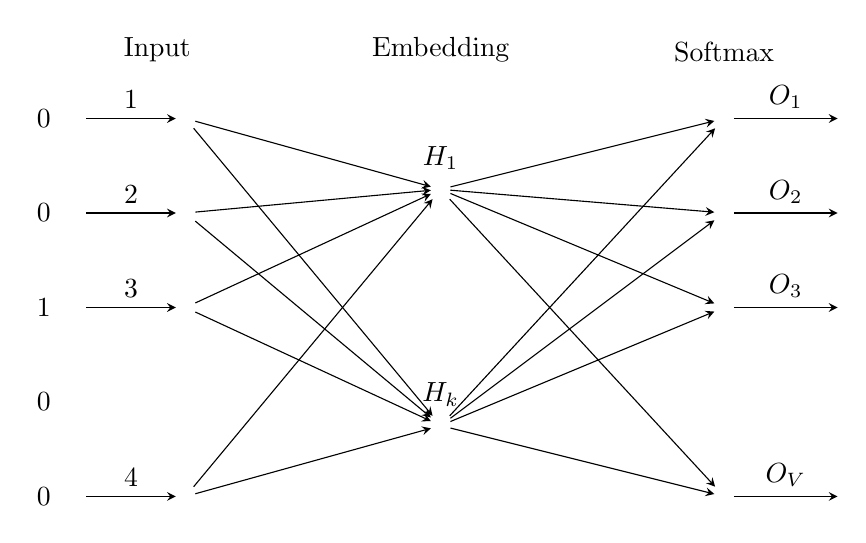
\begin{tikzpicture}[x=1.8cm, y=1.2cm, >=stealth]

\foreach \m/\l [count=\y] in {0, 0 , 1, 0 ,0}
  \node [every neinput/.try, neinput \m/.try] (input-\m) at (-0.8, 2.5-\y) {$\m$};
  
\foreach \m/\l [count=\y] in {1,2,3,missing,4}
  \node [every neuron/.try, neuron \m/.try] (input-\m) at (0.2,2.5-\y) {};

\foreach \m [count=\y] in {1,missing,2}
  \node [every neuron/.try, neuron \m/.try ] (hidden-\m) at (2,2-\y*1.25) {};

\foreach \m [count=\y] in {1,2, 3, missing,4}
  \node [every neuron/.try, neuron \m/.try ] (output-\m) at (4,2.5-\y) {};

\foreach \l [count=\i] in {1,2,3,V}
  \draw [<-] (input-\i) -- ++(-0.7,0)
    node [above, midway] {$\i$};

\foreach \l [count=\i] in {1, k}
  \node [above] at (hidden-\i.north) {$H_\l$};

\foreach \l [count=\i] in {1,2, 3, V}
  \draw [->] (output-\i) -- ++(0.8,0)
    node [above, midway] {$O_\l$};

\foreach \i in {1,...,4}
  \foreach \j in {1,...,2}
    \draw [->] (input-\i) -- (hidden-\j);

\foreach \i in {1,...,2}
  \foreach \j in {1,...,4}
    \draw [->] (hidden-\i) --(output-\j);

\foreach \l [count=\x from 0] in {Input, Embedding, Softmax}
  \node [align=center, above] at (\x*2,2) {\l };

\end{tikzpicture}

A vocabulary is fed into the nerual network using one-hot encoding methods. For a vocabulary of size V, the input vector is of size 1xV

\end{frame}

\section{POS; NER and other NLP probelms}
\begin{frame}
\frametitle{Parts of Speech}
\begin{itemize}
\item Parts-of-speech (POS): noun, verb, pronoun, preposition, adverb, conjunction, participle, and article
\item For example: Can (modal) you (personal pronoun) buy (verb) me (personal pronoun) a (determiner) tea (proper noun)?
\item POS reveal the property of a word and its neighbors

\end{itemize}
\end{frame}

\begin{frame}

\frametitle{English Penn Treebank part-of-speech Tagset}

An important tagset for English is the 45-tag Penn Treebank tagset. 

\vspace{1cm}

\url{https://www.ling.upenn.edu/courses/Fall_2003/ling001/penn_treebank_pos.html}

\end{frame}

%% normal frame
\section{HMM}
\subsection{}


\begin{frame}
    \frametitle{Hidden Markov Model}
 
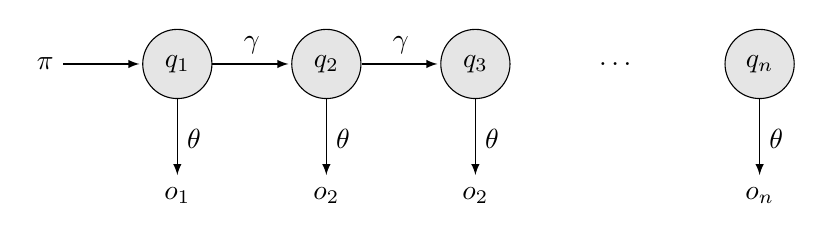
\begin{tikzpicture}
        % Setup the style for the states
        \tikzset{node style/.style={state, 
                                    fill=gray!20!white,
                                    circle}}
    
        \node[node style]               (n0)  {$q_1$};
        \node[node style, right=of n0]  (n1)  {$q_2$};
        \node[node style, right=of n1]  (n2)  {$q_3$};
        \node[draw=none, right=of n2] 	(n3) {$\dots$};
        \node[node style, right=of n3] 	(n) {$q_n$};

        % Draw empty nodes so we can connect them with arrows
        \node[draw=none, left=of n0] (pi0) {$\pi$};

        \node[draw=none, below=of n0] (q0) {$o_1$};
        \node[draw=none, below=of n1] (q1) {$o_2$};
        \node[draw=none, below=of n2] (q2) {$o_2$};
        \node[draw=none, below=of n] (qn) {$o_n$};


    \draw[>=latex,
          auto=left,
          every loop]
          (pi0) edge node {} (n0)
		  (n0) edge node {$\gamma$} (n1)
		  (n1) edge node {$\gamma$} (n2)
		  (n0) edge node {$\theta$} (q0)
		  (n1) edge node {$\theta$} (q1)
		  (n2) edge node {$\theta$} (q2)
		  (n) edge node {$\theta$} (qn);


\end{tikzpicture}

\end{frame}

\begin{frame}
\frametitle{Hidden Markov Model}

\begin{align*}
&p(o_1, o_2, ..., o_T, q_1, q_2, ..., q_T)\\
&=p(q_1, q_2, ..., q_T)\prod_{i=1}^{T} p(o_i\mid q_i)\\
&=p(q_T\mid q_1, q_2, ..., q_{T-1})p(q_1, q_2, ..., q_{T-1})\prod_{i=1}^{T}p(o_i\mid q_i)\\
&=p(q_T\mid q_{T-1})p(q_1, q_2, ..., q_{T-1})\prod_{i=1}^{T} p(o_i\mid q_i)\\
&=\prod_{i=1}^{T} p(q_i|q_{i-1})\prod_{i=1}^{T} p(o_i\mid q_i)
\end{align*}

\end{frame}
\begin{frame}
At each time step, the probability of being in state j after seeing the first t observations, given the automaton $\lambda$ can be calculated as 

$$
\alpha_{t}(j)=\sum_{i=1}^{N}\alpha_{t-1}(i) \gamma_{ij} \theta_j(o_t),
$$
where
$$ 1 \leq t\leq  T, 1\leq j \leq N
$$

where $\theta_j(o_t)$ is the likelihood of observing $o_t$ given the current state is $j$, $\lambda_{ij}$ is the probability of transition from hidden state $i$ to  hidden state $j$. The probability of state $q_j$ at time $t$ is a summation over all paths that could lead to the state. Therefore, the probability of seeing the observed sequence can be calculated as 
$$
P(o\mid \lambda)=\sum_{i=1}^{N}\alpha_{T}(i)
$$
\end{frame}
\begin{frame}
    \frametitle{Hidden Markov Model}
 
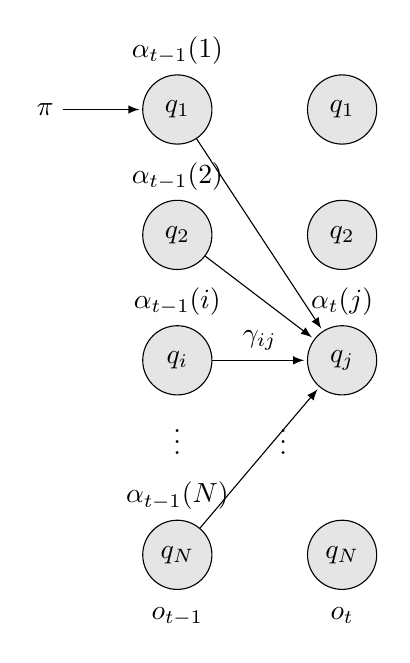
\begin{tikzpicture}
        % Setup the style for the states
        \tikzset{node style/.style={state, 
                                    fill=gray!20!white,
                                    node distance=0.7cm and 1.2cm,
                                    circle,
                                    scale=1}}
    
        \node[node style, label=above:$\alpha_{t-1}(1)$]               (n0)  {$q_1$};
        \node[node style, below=of n0, label=above:$\alpha_{t-1}(2)$]  (n1)  {$q_2$};
        \node[node style, below=of n1, label=above:$\alpha_{t-1}(i)$]  (n2)  {$q_i$};
        \node[draw=none, below= 0.1cm of n2] 	(n3) {$\vdots$};
        \node[node style, below=of n3, label=above:$\alpha_{t-1}(N)$] 	(n) {$q_N$};

        \node[node style, right=of n0]  (m0)  {$q_1$};
        \node[node style, right=of n1]  (m1)  {$q_2$};
        \node[node style, right=of n2, label=above:$\alpha_{t}(j)$]  (m2)  {$q_j$};
        \node[draw=none, right=of n3]  (m3)  {$\vdots$};
        \node[node style, right=of n]  (m)  {$q_N$};


        % Draw empty nodes so we can connect them with arrows
        \node[draw=none, left=of n0] (pi0) {$\pi$};


        \node[draw=none, below= 0.1 cm of n] (qn) {$o_{t-1}$};
        \node[draw=none, below=0.1 cm of m] (qm) {$o_{t}$};


    \draw[>=latex,
          auto=left,
          every loop]
          (pi0) edge node {} (n0)
		  (n0) edge node {} (m2)
		  (n1) edge node {} (m2)
		  (n2) edge node {$\gamma_{ij}$} (m2)
		  (n) edge node {} (m2);



\end{tikzpicture}

\end{frame}

\begin{frame}
	\frametitle{HMM: Viterbi Algorithm}
Given that we know the HMM $\lambda=(\Gamma, \Theta)$ and an observed squence of $O=o_1, o_2, ... o_T$, find the most probable sequence of states $Q=q_1, q_2, q_2, ..., q_T$. 

The viterbi path probablity: the probability of the most probable path that leads to the jth state at time step t. Denoted as 

$$
\nu_t(j)=\max\limits_{q1, q2, q3, ...q_{t-1}}p(q_1, q_2, ... q_{t-1}, q_t=j, o_1, o_2, ..., o_t\mid \lambda)
$$

We can calculate the viterbi path probabilty of being at state $q_j$ at time $t$  as 
$$
\nu_{t}(j)=\max\limits_{i=1}^{N}\nu_{t-1}(i)\gamma_{ij}\theta_j(o_t)
$$

The Viterbie Algorithm needs to back trace the most likely state sequence that leads to the probability. $bt_t(j)$, which can be found by 

$$
bt_t(j)=\argmax\limits_{i=1}^{N}\nu_{t-1}(i)\gamma_{ij}\theta_j(o_t)
$$


\end{frame}

\begin{frame}

\frametitle{HMM: Backward Algorithm}
Denote the probability of seeing the observation after $t+1$ as $o_{t+1} , o_{t+2}, ...o_{T}$, given that we are at state $j$ at time t. 

$$
\beta_t(j)=p(o_{t+1}, o_{t+2}, ..., o_T\mid q_{t}=j, \lambda)
$$

The $\beta_t(j)$ can be expressed as the following formula

\begin{align*}
\beta_{t}(j)
&=\sum\limits_{k=1}^{N}\gamma_{jk}\theta_{k}(o_{t+1})p(o_{t+2}, o_{t+3}, ..., o_T\mid q_{t+1}=k, \lambda)\\
&=\sum\limits_{k=1}^{N}\gamma_{jk}\theta_{k}(o_{t+1})\beta_{t+1}(k)
\end{align*}
\end{frame}

\begin{frame}
The transition probability of going from $ith$ state at time $t-1$ to $jth$ state at time $t$ can be calculated as

$$
p(O|\lambda)=\sum\limits_{t=1}^N\sum\limits_{j=1}^{N} \alpha_{t}(j)\beta_{t}(j)
$$

$$
p(q_{t}=i, q_{t+1}=j, O \mid \lambda)=\sum\limits_{t=1}^N\sum\limits_{j=1}^{N}\alpha_{t}(i)\gamma_{ij}\theta_{j}(o_{t+1})\beta_{t+1}(j)
$$

\begin{align*}
\hat{\gamma_{ij}}
&=p(q_{t-1}=i, q_t=j, \mid O, \lambda)\\
&=p(q_{t-1}=i, q_t=j, O \mid \lambda)/p(O \mid \lambda)\\
&=\frac{\sum\limits_{t=1}^N\alpha_{t}(i)\gamma_{ij}\theta_{j}(o_{t+1})\beta_{t+1}(j)}{\sum\limits_{t=1}^N\sum\limits_{j=1}^{N} \alpha_{t}(j)\beta_{t}(j)}
\end{align*}
\end{frame}

\begin{frame}
Similarly, to calculate the emission probability $\theta_j(o_t)$

\begin{align*}
\eta_t(j)
&=p(q_t=j \mid O, \lambda))\\
&=\frac{p(q_t=j, O \mid \lambda)}{p(O \mid \lambda)}\\
&=\frac{\alpha_t(j)\beta_t(j)}{\sum\limits_{j=1}^{N}\alpha_t(j)\beta_t(j)}
\end{align*}


The emission probability can be estimated as 
$$
\hat{b_j}(k)=\frac{\sum\limits_{t=1, s.t. o_t=k}^{T}\eta_t(j)}{\sum\limits_{t=1}^{T}\eta_t(j)}
$$

\end{frame}


\begin{frame}
\frametitle{Name Entity Recognition (NER)}
\begin{itemize}
\item NER labels words in a texts that are names of things e.g. person, organization, money amount, gene/protein names
\item John (person) Lee (person) is the chief of CBSE (organization). 
\end{itemize}
\end{frame}
\end{document}
